\chapter{Representación.}\label{cap:capitulo3}

En este capítulo entraremos en detalle de la representación de los distintos elementos que componen el generador. Repasaremos el concepto de \emph{mapa de tiles} de nuevo. Analizaremos la representación lógica y física necesaria con el objetivo de establecer un modelo claro para las habitaciones y el mapa que usaremos posteriormente para la construcción del sistema de generación.


En nuestro contexto, disponemos de dos tipos de entidades:

\begin{itemize}
	\item \emph{Habitaciones} que compondrán el mapa.
	\item \emph{Mapa} o escenario donde se desarrolla el juego, compuesto por habitaciones. Posee algunos elementos ausentes en las habitaciones.
\end{itemize}

Es importante tener claro el aspecto de la representación de las entidades que se utilizarán en el sistema, ya que el mismo se construirá en base a lo que se detalle en la representación.

\section{Topología.}

Como se ha repetido varias veces anteriormente, usaremos un \emph{mapa de tiles} para la representación del escenario. Esto implica que los modelos tanto de las habitaciones como del propio mapa, han de mantener una matriz para la representación física. En la figura~~\ref{fig:memtiles} podemos ver la representación en memoria como una matriz de un mapa de tiles. En la figura~\ref{fig:graftiles} se observa la representación gráfica. Se puede comprobar la relación directa entre ambas representaciones.


\begin{figure}[h]
\centering
{
	$
\begin{matrix}
	0 & 1 & 1 & 1 & 0 \\
	0 & 1 & 0 & 1 & 1 \\
	1 & 1 & 0 & 0 & 1 \\
	1 & 0 & 0 & 0 & 1 \\
	1 & 1 & 1 & 1 & 1
\end{matrix}
$
}
\caption{Representación en memoria de un mapa de tiles
\label{fig:memtiles}
}
\end{figure}

\begin{figure}[t]
\centering
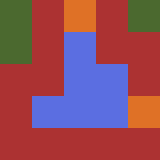
\includegraphics[scale=1]{img/graftiles}
\caption{Representación gráfica de un mapa de tiles
\label{fig:graftiles}}
\end{figure}

En principio, los tipos de tile que se han considerado son los siguientes:

\begin{itemize}
	\item \textcolor{red}{\emph{Tile pared}}. Representa una porción de geometría sólida infranqueable. A la hora de colocar habitaciones, habrá que añadir un mecanismo para evitar el solapamiento entre tiles sólidos de entidades distintas.
	\item \textcolor{blue}{\emph{Tile interior}}. Representa una porción de geometría traspasable. A igual que el tile sólido, habrá que evitar solapamiento con tiles pertenecientes a otras entidades (habitaciones o el mapa).
	\item \textcolor{OliveGreen}{\emph{Tile exterior}}. Representa una porción de geometría traspasable \emph{externa} a la habitación. Este tipo de tiles sí que puede solaparse con tiles pertenecientes a otras entidades.
	\item \textcolor{orange}{\emph{Tile puerta}}. Representa una conexión entre dos habitaciones. No podrá solaparse, pero si traspasarse para permitir el cruce entre habitaciones.
\end{itemize}

En la figura~~\ref{fig:proptiles} se ve un resumen de las propiedades inherentes a cada tipo de tile.

\begin{figure}[h]
\centering
{
\begin{tabular}{|c|c|c|}
\hline
		& Sólido 		& Solapable 	\\
\hline
Pared 	&  \checkmark  	&  X  			\\ \hline
Interno &  X			&  X  			\\ \hline
Externo &  X  			&  \checkmark  	\\ \hline
Puerta  &  X  			&  X 		 	\\ \hline
\end{tabular}
}
\caption{Propiedades de los tiles
\label{fig:proptiles}
}

\end{figure}



Con todo ésto, ya tenemos clara la representación física de los distintos elementos implicados en el sistema de generación. Ahora, entraremos en detalle con elementos específicos para el mapa y la habitación, que principalmente nos serán necesarios para algunas optimizaciones y llevar a cabo la lógica del generador.

Más adelante veremos un tipo de tile especial (tile tipo \emph{puerta}) en el que nos apoyaremos para la conexión entre habitaciones.

\section{Habitaciones.}

Analizaremos los elementos relevantes para la representación de las habitaciones. Atendiendo a la especificación de que las habitaciones \emph{se pueden repetir}, se ha dividido la representación en dos componentes:

\begin{itemize}
	\item \emph{Prefab}. Representación que engloba los elementos comunes para un modelo de habitación. Sirve, entre otras cosas, para almacenar solamente un mapa de tiles por modelo de habitación.
	\item \emph{Instancia}. Representación específica para una concretización o instancia de un modelo de habitación o prefab. Contendrá información sobre la posición de una habitación en el mapa y las puertas.
\end{itemize}

Ésto nos permite un ahorro de memoria, ya que guardamos información común a muchas habitaciones en un solo modelo, y procesamiento, que veremos en detalle en el capítulo 4 (INSERTAENLACE).

\subsection{Puertas potenciales.}

Antes de abarcar los dos componentes empleados para representar las habitaciones, vamos a introducir el concepto de \emph{puerta potencial}, que será necesario para explicar una de las motivaciones del \emph{prefab} (además de tener que mantener solo un mapa de tiles por modelo).



\subsection{Prefabs.}

\subsection{Instancias.}

\section{Mapa.}

